\documentclass{article}

\usepackage{graphicx}
\usepackage{tikz}
\usepackage{tikzsymbols}
\usetikzlibrary{calc,patterns,shapes.geometric}
\pagestyle{empty}
\usepackage[margin=0pt]{geometry}
\geometry{papersize={14in,12in}}

\def\centerarc[#1](#2)(#3:#4:#5){\draw[#1] ($(#2)+({#5*cos(#3)},{#5*sin(#3)})$) arc (#3:#4:#5);}

\begin{document}
	\begin{figure}
		\centering
		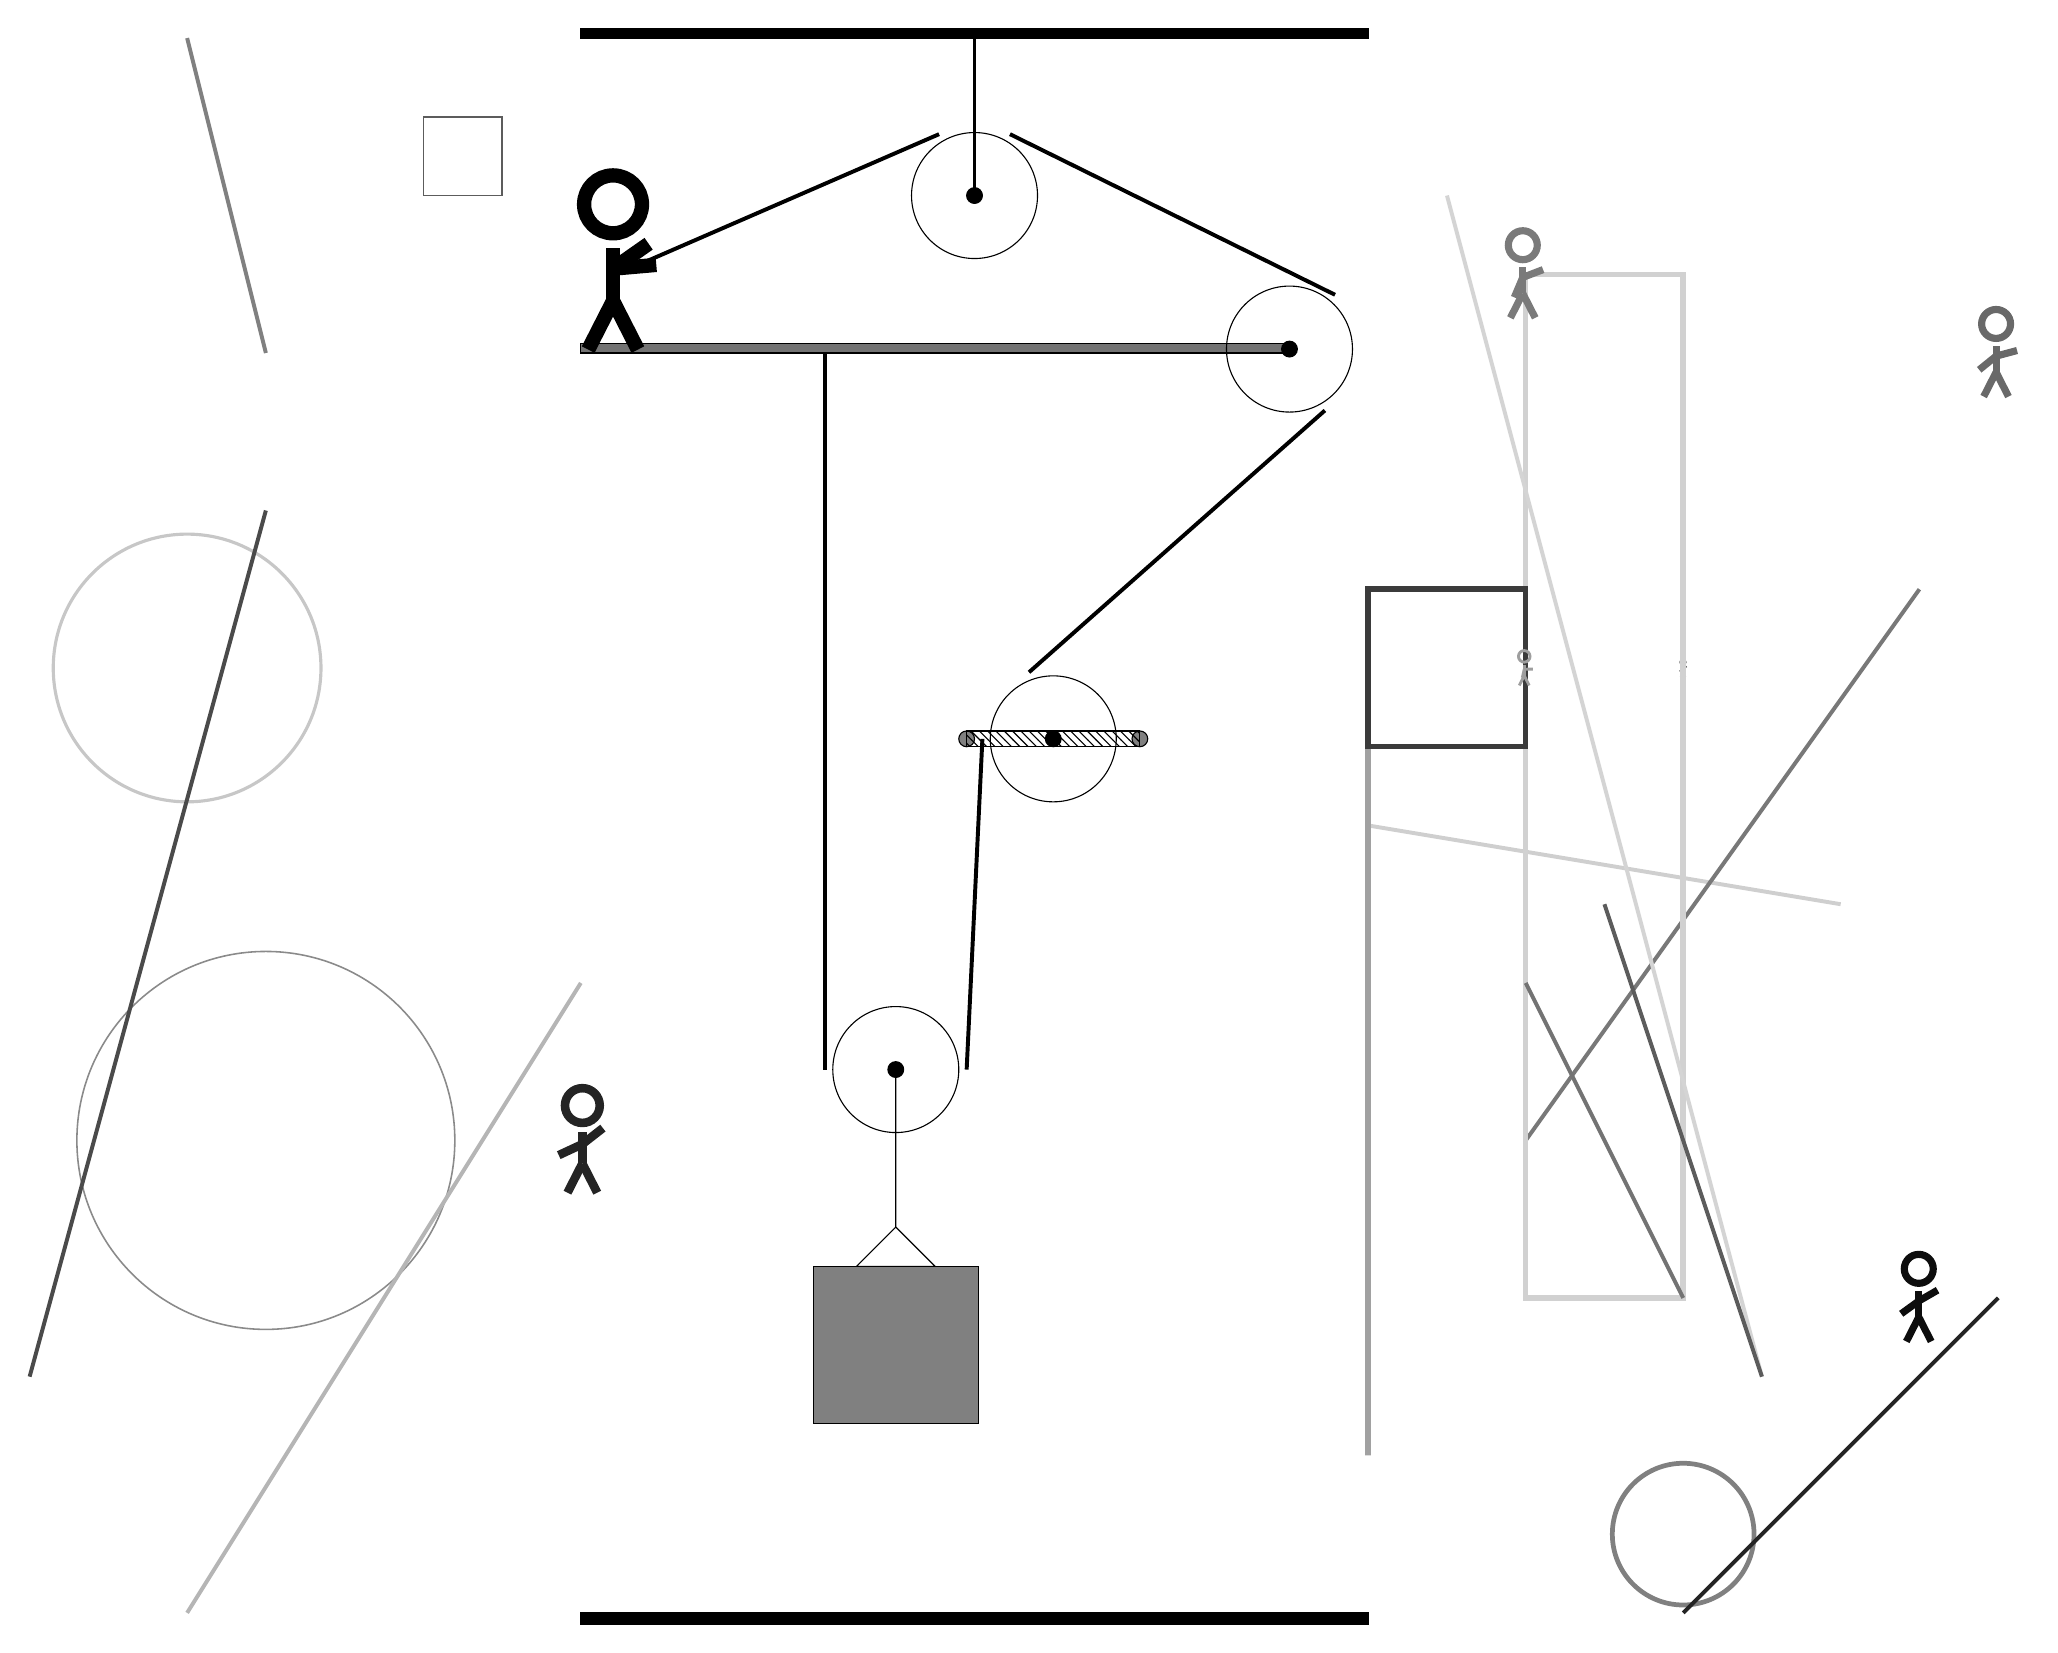
\begin{tikzpicture}
			%%%%% START %%%%%
			
			\draw[fill=black] (-2, 18) rectangle (8, 18.125);
			
			\draw[line width=0.5mm, color=black!50](-7, 18) -- (-6, 14);
			
			\node[line width=0.3mm, color=black!86] at (-2, 4) {\Strichmaxerl[6][25][38]};
			\node[line width=0.4mm, color=black!62] at (12, 10) {\Strichmaxerl[1][39][29]};
			\draw[line width=0.5mm, color=black!19](8, 8) -- (14, 7);
			\node[line width=0.5mm, color=black!59] at (16, 14) {\Strichmaxerl[5][39][15]};
			
			\draw[line width=0.5mm, color=black!53](10, 4) -- (15, 11);
			
			\draw[line width=0.7mm, color=black!18] (10, 2) rectangle (12, 15);
			\draw[line width=0.7mm, color=black!37] (8, 0) rectangle (8, 11);
			\draw[line width=0.5mm, color=black!17](9, 16) -- (13, 1);
			\node[line width=0.5mm, color=black!95] at (15, 2) {\Strichmaxerl[5][36][30]};
			
			\draw [line width=0.4mm, color=black!40](-5, 10) circle (0.0);
			
			\draw[line width=0.7mm, color=black!77] (10, 11) rectangle (8, 9);
			\draw [line width=0.4mm, color=black!22](-7, 10) circle (1.7);
			
			\draw [line width=0.6mm, color=black!50](12, -1) circle (0.9);
			\node[line width=0.6mm, color=black!38] at (10, 10) {\Strichmaxerl[2][77][1]};
			\draw[line width=0.5mm, color=black!86](12, -2) -- (16, 2);
			\draw[line width=0.5mm, color=black!64](11, 7) -- (13, 1);
			\draw[line width=0.5mm, color=black!55](12, 2) -- (10, 6);
			\draw [line width=0.2mm, color=black!46](-6, 4) circle (2.4);
			\node[line width=0.3mm, color=black!52] at (10, 15) {\Strichmaxerl[5][67][21]};
			\draw[line width=0.2mm, color=black!64] (-4, 16) rectangle (-3, 17);
			
			\draw[line width=0.5mm, color=black!71](-6, 12) -- (-9, 1);
			
			\draw[line width=0.5mm, color=black!29](-2, 6) -- (-7, -2);
			
			\draw[fill=black!55] (-2, 14) rectangle (7, 14.125);
			
			\draw (2, 4.9) circle (0.8);
			\draw[fill=black] (2, 4.9) circle (0.1);
			
			\draw (7, 14.05) circle (0.8);
			\draw[fill=black] (7, 14.05) circle (0.1);
			
			\draw[fill=white](4, 9.1) circle (0.8);
			\draw[fill=black] (4, 9.1) circle (0.1);
			\draw[fill=black!50] (2.9, 9.1) circle (0.1);
			\draw[fill=black!50] (5.1, 9.1) circle (0.1);
			\draw[pattern=north west lines, pattern color=black] (2.9, 9.2) rectangle (5.1, 9.0);
			
			\draw (3, 16) circle (0.8);
			\draw[fill=black] (3, 16) circle (0.1);
			\draw[line width=0.5mm] (3, 16) -- (3, 18);
			
			\draw (2, 4.9) -- (2, 2.9) -- (1.5, 2.4) -- (2.5, 2.4) -- (2, 2.9);
			\draw[fill=black!50] (0.95, 2.4) rectangle (3.05, 0.4);
			
			\draw[line width=0.5mm] (1.1, 14) -- (1.1, 4.9);
			\centerarc[line width=0.5mm](2, 4.9)(180:360:0.9);
			\draw[line width=0.5mm](2.9, 4.9) -- (3.1, 9.1);
			\centerarc[line width=0.5mm](4, 9.1)(110:180:0.9);
			\draw[line width=0.5mm](3.6922, 9.9457) -- (7.45, 13.2706);
			\centerarc[line width=0.5mm](7, 14.05)(-60:50:0.9);
			\draw[line width=0.5mm](7.5785, 14.7394) -- (3.45, 16.7794);
			\centerarc[line width=0.5mm](3, 16)(60:120:0.9);
			\draw[line width=0.5mm](2.55, 16.7794) -- (-1.2, 15.15);
			
			\node at (-1.5, 15.15) {\Strichmaxerl[10][-175][35]};
			
			\draw[fill=black] (-2, -2) rectangle (8, -2.15);
			
			%%%%% END %%%%%
		\end{tikzpicture}
	\end{figure}	
\end{document}